\documentclass[12pt]{article}
\usepackage{graphicx}
\begin{document}

\section{Problem}
SIR model for a single class of population
with respect to time t and variables $[S, I, R]$ for constant population



\begin{eqnarray}
\frac{dS}{dt} &=& - \beta  S I \\
\frac{dI}{dt} &= &\beta  S I -  \gamma I \\
\frac{dR}{dt} &=& \gamma I
\end{eqnarray}

\begin{itemize}
\item $[S, I, R]$: values of the variables (ratio of suceptibles, infectious and recovered fraction of the population)
\item $t$: time (not used because autonomous ODE)
\item $\beta$ : transmission coefficient.
\item $\gamma$ : healing rate.
\end{itemize}

\section{Results}

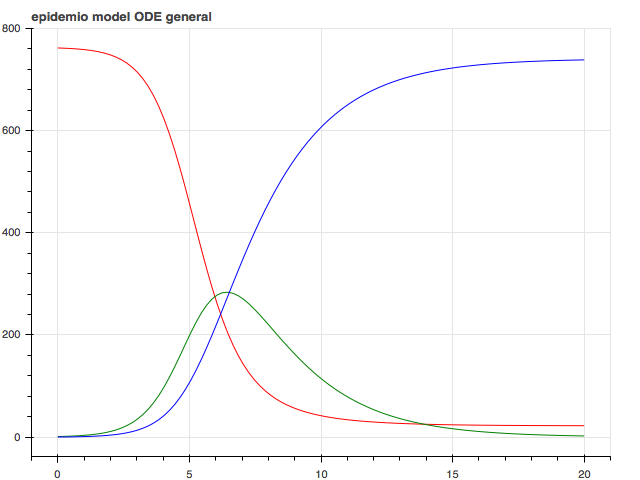
\includegraphics[height=7cm]{figure.png}

\end{document}
